\documentclass[twoside]{book}

% Packages required by doxygen
\usepackage{fixltx2e}
\usepackage{calc}
\usepackage{doxygen}
\usepackage[export]{adjustbox} % also loads graphicx
\usepackage{graphicx}
\usepackage[utf8]{inputenc}
\usepackage{makeidx}
\usepackage{multicol}
\usepackage{multirow}
\PassOptionsToPackage{warn}{textcomp}
\usepackage{textcomp}
\usepackage[nointegrals]{wasysym}
\usepackage[table]{xcolor}

% Font selection
\usepackage[T1]{fontenc}
\usepackage[scaled=.90]{helvet}
\usepackage{courier}
\usepackage{amssymb}
\usepackage{sectsty}
\renewcommand{\familydefault}{\sfdefault}
\allsectionsfont{%
  \fontseries{bc}\selectfont%
  \color{darkgray}%
}
\renewcommand{\DoxyLabelFont}{%
  \fontseries{bc}\selectfont%
  \color{darkgray}%
}
\newcommand{\+}{\discretionary{\mbox{\scriptsize$\hookleftarrow$}}{}{}}

% Page & text layout
\usepackage{geometry}
\geometry{%
  a4paper,%
  top=2.5cm,%
  bottom=2.5cm,%
  left=2.5cm,%
  right=2.5cm%
}
\tolerance=750
\hfuzz=15pt
\hbadness=750
\setlength{\emergencystretch}{15pt}
\setlength{\parindent}{0cm}
\setlength{\parskip}{3ex plus 2ex minus 2ex}
\makeatletter
\renewcommand{\paragraph}{%
  \@startsection{paragraph}{4}{0ex}{-1.0ex}{1.0ex}{%
    \normalfont\normalsize\bfseries\SS@parafont%
  }%
}
\renewcommand{\subparagraph}{%
  \@startsection{subparagraph}{5}{0ex}{-1.0ex}{1.0ex}{%
    \normalfont\normalsize\bfseries\SS@subparafont%
  }%
}
\makeatother

% Headers & footers
\usepackage{fancyhdr}
\pagestyle{fancyplain}
\fancyhead[LE]{\fancyplain{}{\bfseries\thepage}}
\fancyhead[CE]{\fancyplain{}{}}
\fancyhead[RE]{\fancyplain{}{\bfseries\leftmark}}
\fancyhead[LO]{\fancyplain{}{\bfseries\rightmark}}
\fancyhead[CO]{\fancyplain{}{}}
\fancyhead[RO]{\fancyplain{}{\bfseries\thepage}}
\fancyfoot[LE]{\fancyplain{}{}}
\fancyfoot[CE]{\fancyplain{}{}}
\fancyfoot[RE]{\fancyplain{}{\bfseries\scriptsize Generated by Doxygen }}
\fancyfoot[LO]{\fancyplain{}{\bfseries\scriptsize Generated by Doxygen }}
\fancyfoot[CO]{\fancyplain{}{}}
\fancyfoot[RO]{\fancyplain{}{}}
\renewcommand{\footrulewidth}{0.4pt}
\renewcommand{\chaptermark}[1]{%
  \markboth{#1}{}%
}
\renewcommand{\sectionmark}[1]{%
  \markright{\thesection\ #1}%
}

% Indices & bibliography
\usepackage{natbib}
\usepackage[titles]{tocloft}
\setcounter{tocdepth}{3}
\setcounter{secnumdepth}{5}
\makeindex

% Hyperlinks (required, but should be loaded last)
\usepackage{ifpdf}
\ifpdf
  \usepackage[pdftex,pagebackref=true]{hyperref}
\else
  \usepackage[ps2pdf,pagebackref=true]{hyperref}
\fi
\hypersetup{%
  colorlinks=true,%
  linkcolor=blue,%
  citecolor=blue,%
  unicode%
}

% Custom commands
\newcommand{\clearemptydoublepage}{%
  \newpage{\pagestyle{empty}\cleardoublepage}%
}

\usepackage{caption}
\captionsetup{labelsep=space,justification=centering,font={bf},singlelinecheck=off,skip=4pt,position=top}

%===== C O N T E N T S =====

\begin{document}

% Titlepage & ToC
\hypersetup{pageanchor=false,
             bookmarksnumbered=true,
             pdfencoding=unicode
            }
\pagenumbering{alph}
\begin{titlepage}
\vspace*{7cm}
\begin{center}%
{\Large Інформаційна система обліку площу будівель }\\
\vspace*{1cm}
{\large Generated by Doxygen 1.8.14}\\
\end{center}
\end{titlepage}
\clearemptydoublepage
\pagenumbering{roman}
\tableofcontents
\clearemptydoublepage
\pagenumbering{arabic}
\hypersetup{pageanchor=true}

%--- Begin generated contents ---
\chapter{Hierarchical Index}
\section{Class Hierarchy}
This inheritance list is sorted roughly, but not completely, alphabetically\+:\begin{DoxyCompactList}
\item \contentsline{section}{House}{\pageref{class_house}}{}
\item \contentsline{section}{Room}{\pageref{class_room}}{}
\begin{DoxyCompactList}
\item \contentsline{section}{Curc\+Room}{\pageref{class_curc_room}}{}
\item \contentsline{section}{Rect\+Room}{\pageref{class_rect_room}}{}
\end{DoxyCompactList}
\end{DoxyCompactList}

\chapter{Class Index}
\section{Class List}
Here are the classes, structs, unions and interfaces with brief descriptions\+:\begin{DoxyCompactList}
\item\contentsline{section}{\mbox{\hyperlink{class_curc_room}{Curc\+Room}} }{\pageref{class_curc_room}}{}
\item\contentsline{section}{\mbox{\hyperlink{class_house}{House}} }{\pageref{class_house}}{}
\item\contentsline{section}{\mbox{\hyperlink{class_rect_room}{Rect\+Room}} }{\pageref{class_rect_room}}{}
\item\contentsline{section}{\mbox{\hyperlink{class_room}{Room}} }{\pageref{class_room}}{}
\end{DoxyCompactList}

\chapter{Class Documentation}
\hypertarget{class_curc_room}{}\section{Curc\+Room Class Reference}
\label{class_curc_room}\index{Curc\+Room@{Curc\+Room}}
Inheritance diagram for Curc\+Room\+:\begin{figure}[H]
\begin{center}
\leavevmode
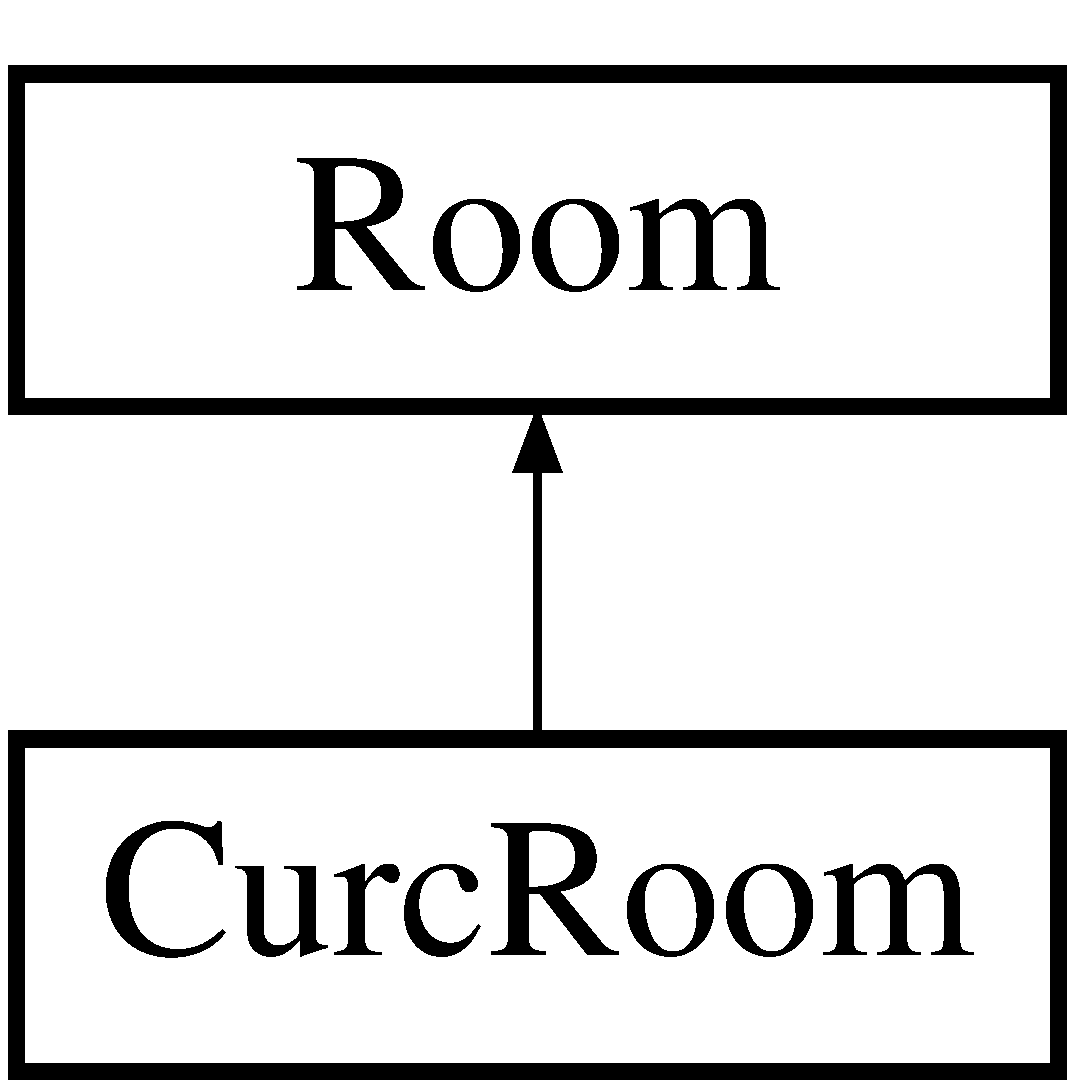
\includegraphics[height=2.000000cm]{class_curc_room}
\end{center}
\end{figure}
\subsection*{Public Member Functions}
\begin{DoxyCompactItemize}
\item 
\mbox{\Hypertarget{class_curc_room_a768566b7c9eebf909990302525836f0e}\label{class_curc_room_a768566b7c9eebf909990302525836f0e}} 
{\bfseries Curc\+Room} (double x, double y, double radius)
\item 
\mbox{\Hypertarget{class_curc_room_a83b8ca5d1147018a4acbd1db8d66cff3}\label{class_curc_room_a83b8ca5d1147018a4acbd1db8d66cff3}} 
double {\bfseries GetX} () const
\item 
\mbox{\Hypertarget{class_curc_room_ac5062f9fc34fd29fd7c3548ec4cede51}\label{class_curc_room_ac5062f9fc34fd29fd7c3548ec4cede51}} 
double {\bfseries GetY} () const
\item 
\mbox{\Hypertarget{class_curc_room_a63e10278169feffef1ecba77cb66a7be}\label{class_curc_room_a63e10278169feffef1ecba77cb66a7be}} 
double {\bfseries Get\+Radius} () const
\item 
virtual double \mbox{\hyperlink{class_curc_room_a0026b4be5fc20d3d1e701d4c5acdf994}{Get\+Square}} () const override
\end{DoxyCompactItemize}


\subsection{Member Function Documentation}
\mbox{\Hypertarget{class_curc_room_a0026b4be5fc20d3d1e701d4c5acdf994}\label{class_curc_room_a0026b4be5fc20d3d1e701d4c5acdf994}} 
\index{Curc\+Room@{Curc\+Room}!Get\+Square@{Get\+Square}}
\index{Get\+Square@{Get\+Square}!Curc\+Room@{Curc\+Room}}
\subsubsection{\texorpdfstring{Get\+Square()}{GetSquare()}}
{\footnotesize\ttfamily double Curc\+Room\+::\+Get\+Square (\begin{DoxyParamCaption}{ }\end{DoxyParamCaption}) const\hspace{0.3cm}{\ttfamily [override]}, {\ttfamily [virtual]}}

Square Calculating Method 

Implements \mbox{\hyperlink{class_room_a031b559260949b3fa9e27053aaf602f5}{Room}}.



The documentation for this class was generated from the following files\+:\begin{DoxyCompactItemize}
\item 
Curc\+Room.\+h\item 
Curc\+Room.\+cpp\end{DoxyCompactItemize}

\hypertarget{class_house}{}\section{House Class Reference}
\label{class_house}\index{House@{House}}
\subsection*{Public Member Functions}
\begin{DoxyCompactItemize}
\item 
\mbox{\Hypertarget{class_house_a34103c16773b7b0fc825a91f463e82fb}\label{class_house_a34103c16773b7b0fc825a91f463e82fb}} 
void {\bfseries add\+Room} (\mbox{\hyperlink{class_room}{Room}} room)
\item 
\mbox{\Hypertarget{class_house_ab3effdfacda266ced2f1e847b96e49e4}\label{class_house_ab3effdfacda266ced2f1e847b96e49e4}} 
void {\bfseries delete\+Room} (int index)
\item 
\mbox{\Hypertarget{class_house_ab7f00c3b447a9ed771e18cfb907e9585}\label{class_house_ab7f00c3b447a9ed771e18cfb907e9585}} 
size\+\_\+t {\bfseries get\+Room\+Count} () const
\item 
\mbox{\Hypertarget{class_house_a6e664594b2407ae36294feeafbe8d591}\label{class_house_a6e664594b2407ae36294feeafbe8d591}} 
bool {\bfseries is\+Empty} () const
\item 
\mbox{\Hypertarget{class_house_a024343d1dd5196dca6888a968ce2659a}\label{class_house_a024343d1dd5196dca6888a968ce2659a}} 
double {\bfseries get\+Summury\+Square} () const
\item 
\mbox{\Hypertarget{class_house_aff3fbb1a1b8373f8080fac0130c02ee1}\label{class_house_aff3fbb1a1b8373f8080fac0130c02ee1}} 
void {\bfseries Clear\+All} ()
\end{DoxyCompactItemize}


The documentation for this class was generated from the following files\+:\begin{DoxyCompactItemize}
\item 
House.\+h\item 
House.\+cpp\end{DoxyCompactItemize}

\hypertarget{class_rect_room}{}\section{Rect\+Room Class Reference}
\label{class_rect_room}\index{Rect\+Room@{Rect\+Room}}
Inheritance diagram for Rect\+Room\+:\begin{figure}[H]
\begin{center}
\leavevmode
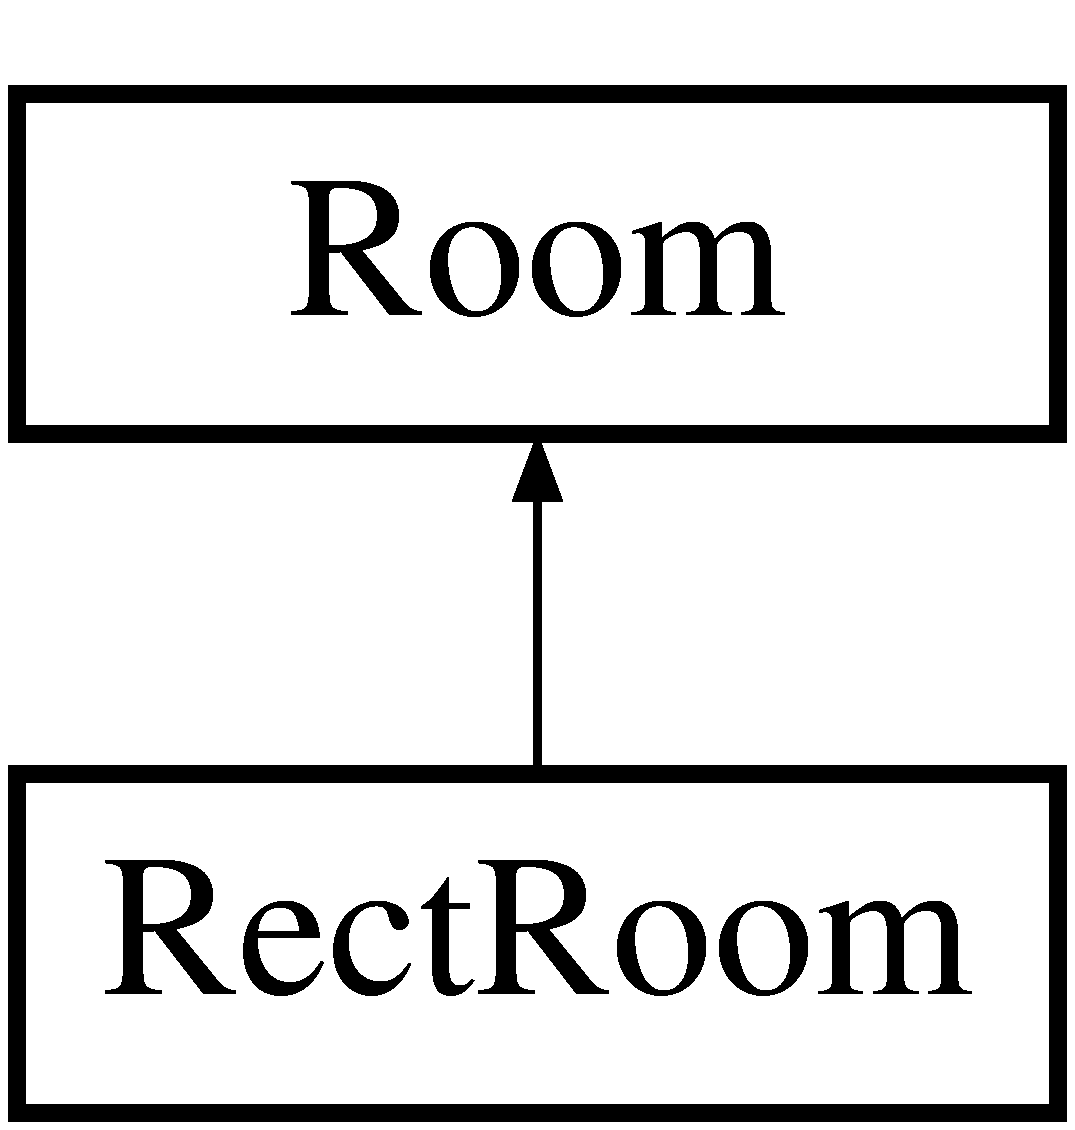
\includegraphics[height=2.000000cm]{class_rect_room}
\end{center}
\end{figure}
\subsection*{Public Member Functions}
\begin{DoxyCompactItemize}
\item 
\mbox{\Hypertarget{class_rect_room_a444fad0f9f4214cc71050aeae4522316}\label{class_rect_room_a444fad0f9f4214cc71050aeae4522316}} 
{\bfseries Rect\+Room} (double x, double y, double width, double height)
\item 
\mbox{\Hypertarget{class_rect_room_aac644aa64bdbd3ed45e04280408d5759}\label{class_rect_room_aac644aa64bdbd3ed45e04280408d5759}} 
double {\bfseries GetX} () const
\item 
\mbox{\Hypertarget{class_rect_room_ac451b16217c726a27a0ca153f4694e89}\label{class_rect_room_ac451b16217c726a27a0ca153f4694e89}} 
double {\bfseries GetY} () const
\item 
\mbox{\Hypertarget{class_rect_room_aab5c14d8e4f9a28535acdd3fb571b5aa}\label{class_rect_room_aab5c14d8e4f9a28535acdd3fb571b5aa}} 
double {\bfseries Get\+Width} () const
\item 
\mbox{\Hypertarget{class_rect_room_aa0ce3fcbdf1d34a94d44cd3b417723bf}\label{class_rect_room_aa0ce3fcbdf1d34a94d44cd3b417723bf}} 
double {\bfseries Get\+Height} () const
\item 
virtual double \mbox{\hyperlink{class_rect_room_a3308e46aa110d1b453d7a80cfbb5b5a2}{Get\+Square}} () const override
\end{DoxyCompactItemize}


\subsection{Member Function Documentation}
\mbox{\Hypertarget{class_rect_room_a3308e46aa110d1b453d7a80cfbb5b5a2}\label{class_rect_room_a3308e46aa110d1b453d7a80cfbb5b5a2}} 
\index{Rect\+Room@{Rect\+Room}!Get\+Square@{Get\+Square}}
\index{Get\+Square@{Get\+Square}!Rect\+Room@{Rect\+Room}}
\subsubsection{\texorpdfstring{Get\+Square()}{GetSquare()}}
{\footnotesize\ttfamily double Rect\+Room\+::\+Get\+Square (\begin{DoxyParamCaption}{ }\end{DoxyParamCaption}) const\hspace{0.3cm}{\ttfamily [override]}, {\ttfamily [virtual]}}

Square Calculating Method 

Implements \mbox{\hyperlink{class_room_a031b559260949b3fa9e27053aaf602f5}{Room}}.



The documentation for this class was generated from the following files\+:\begin{DoxyCompactItemize}
\item 
Rect\+Room.\+h\item 
Rect\+Room.\+cpp\end{DoxyCompactItemize}

\hypertarget{class_room}{}\section{Room Class Reference}
\label{class_room}\index{Room@{Room}}
Inheritance diagram for Room\+:\begin{figure}[H]
\begin{center}
\leavevmode
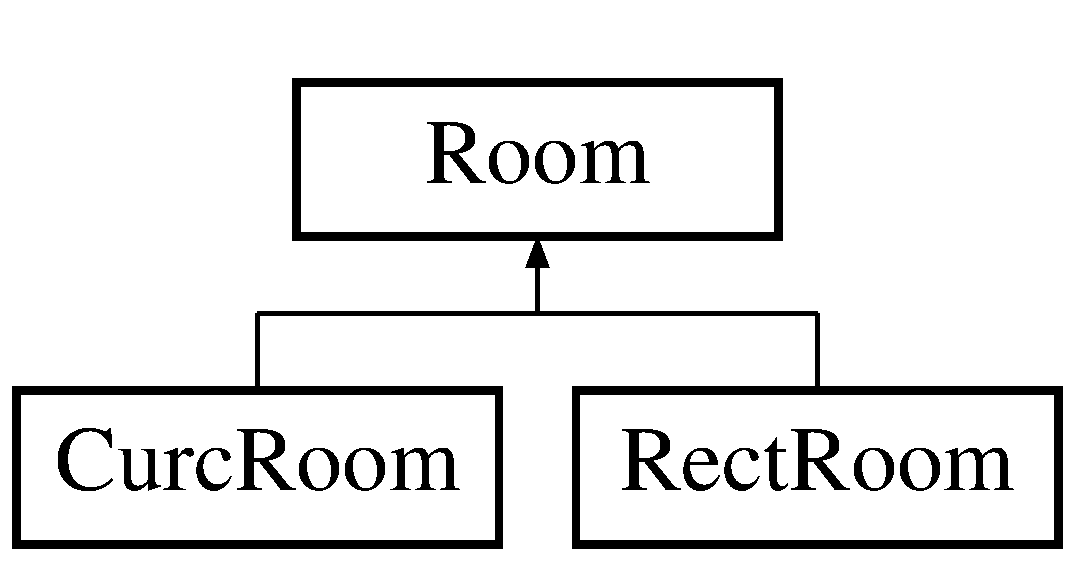
\includegraphics[height=2.000000cm]{class_room}
\end{center}
\end{figure}
\subsection*{Public Member Functions}
\begin{DoxyCompactItemize}
\item 
\mbox{\hyperlink{class_room_ac6ef93a7d9c3e1d624e025058d5f16ff}{Room}} ()
\item 
virtual double \mbox{\hyperlink{class_room_a031b559260949b3fa9e27053aaf602f5}{Get\+Square}} () const =0
\item 
\mbox{\hyperlink{class_room_a67d5da09983cc53097807fd43ba5481a}{$\sim$\+Room}} ()
\item 
void \mbox{\hyperlink{class_room_af7f292c9e840184a5df8525687e87367}{set\+Name}} (std\+::string name)
\item 
std\+::string \mbox{\hyperlink{class_room_a767de198f529425dd4ba81810e44d6e4}{get\+Name}} () const
\end{DoxyCompactItemize}


\subsection{Constructor \& Destructor Documentation}
\mbox{\Hypertarget{class_room_ac6ef93a7d9c3e1d624e025058d5f16ff}\label{class_room_ac6ef93a7d9c3e1d624e025058d5f16ff}} 
\index{Room@{Room}!Room@{Room}}
\index{Room@{Room}!Room@{Room}}
\subsubsection{\texorpdfstring{Room()}{Room()}}
{\footnotesize\ttfamily Room\+::\+Room (\begin{DoxyParamCaption}{ }\end{DoxyParamCaption})}

Constructor of the class \mbox{\Hypertarget{class_room_a67d5da09983cc53097807fd43ba5481a}\label{class_room_a67d5da09983cc53097807fd43ba5481a}} 
\index{Room@{Room}!````~Room@{$\sim$\+Room}}
\index{````~Room@{$\sim$\+Room}!Room@{Room}}
\subsubsection{\texorpdfstring{$\sim$\+Room()}{~Room()}}
{\footnotesize\ttfamily Room\+::$\sim$\+Room (\begin{DoxyParamCaption}{ }\end{DoxyParamCaption})}

Destructor of the class 

\subsection{Member Function Documentation}
\mbox{\Hypertarget{class_room_a767de198f529425dd4ba81810e44d6e4}\label{class_room_a767de198f529425dd4ba81810e44d6e4}} 
\index{Room@{Room}!get\+Name@{get\+Name}}
\index{get\+Name@{get\+Name}!Room@{Room}}
\subsubsection{\texorpdfstring{get\+Name()}{getName()}}
{\footnotesize\ttfamily std\+::string Room\+::get\+Name (\begin{DoxyParamCaption}{ }\end{DoxyParamCaption}) const}

Show room name Method \begin{DoxyReturn}{Returns}
room name 
\end{DoxyReturn}
\mbox{\Hypertarget{class_room_a031b559260949b3fa9e27053aaf602f5}\label{class_room_a031b559260949b3fa9e27053aaf602f5}} 
\index{Room@{Room}!Get\+Square@{Get\+Square}}
\index{Get\+Square@{Get\+Square}!Room@{Room}}
\subsubsection{\texorpdfstring{Get\+Square()}{GetSquare()}}
{\footnotesize\ttfamily virtual double Room\+::\+Get\+Square (\begin{DoxyParamCaption}{ }\end{DoxyParamCaption}) const\hspace{0.3cm}{\ttfamily [pure virtual]}}

Square Calculating Method 

Implemented in \mbox{\hyperlink{class_rect_room_a3308e46aa110d1b453d7a80cfbb5b5a2}{Rect\+Room}}, and \mbox{\hyperlink{class_curc_room_a0026b4be5fc20d3d1e701d4c5acdf994}{Curc\+Room}}.

\mbox{\Hypertarget{class_room_af7f292c9e840184a5df8525687e87367}\label{class_room_af7f292c9e840184a5df8525687e87367}} 
\index{Room@{Room}!set\+Name@{set\+Name}}
\index{set\+Name@{set\+Name}!Room@{Room}}
\subsubsection{\texorpdfstring{set\+Name()}{setName()}}
{\footnotesize\ttfamily void Room\+::set\+Name (\begin{DoxyParamCaption}\item[{std\+::string}]{name }\end{DoxyParamCaption})}

Set room name Method 
\begin{DoxyParams}{Parameters}
{\em name} & room name \\
\hline
\end{DoxyParams}


The documentation for this class was generated from the following files\+:\begin{DoxyCompactItemize}
\item 
Room.\+h\item 
Room.\+cpp\end{DoxyCompactItemize}

%--- End generated contents ---

% Index
\backmatter
\newpage
\phantomsection
\clearemptydoublepage
\addcontentsline{toc}{chapter}{Index}
\printindex

\end{document}
